\documentclass[12pt]{iopart}
\usepackage[a4paper,margin=2.5cm]{geometry}
\usepackage{graphicx}
\usepackage{hyperref}
\usepackage{authblk}
\usepackage{cite}
\usepackage{float}
\usepackage{longtable}
\usepackage{caption}
\usepackage{qrcode}
\captionsetup[longtable]{width=\linewidth, position=bottom}
% --- Eigene Definitionen fehlender Kommandos für iopart ---
\providecommand{\mathbb}[1]{\mathbf{#1}}
\providecommand{\mathcal}[1]{\mathscr{#1}}
\providecommand{\text}[1]{\mbox{#1}}
\providecommand{\implies}{\Rightarrow}
\providecommand{\forall}{\hbox{for all }}
\providecommand{\exists}{\hbox{there exists }}
\providecommand{\quad}{\hskip1em\relax}
\providecommand{\qquad}{\hskip2em\relax}



% --- Titel, Autoren, Affiliations, Open Science, ORCID, Keywords ---
\title{Resonance Field Theory: Axiomatics, Invariants, and Systemic Structure}

\author[1]{Dominic-René Schu\thanks{ORCID: 0000-0003-XXXX-XXXX \\ Email: dominic.rene.schu@gmail.com}}
\affil[1]{Independent Researcher, Germany\\
	\href{https://github.com/DominicReneSchu/public}{https://github.com/DominicReneSchu/public}}

\date{June 2025}

% --- Keywords und Data Availability Statement (IOP verlangt oft beides) ---
\newcommand{\keywords}[1]{\textbf{Keywords:} #1}
\newcommand{\dataavailability}{\textbf{Data and Code Availability:} All data, code, and supplementary materials are openly available at \url{https://github.com/DominicReneSchu/public}.}

% --- Beginn Dokument ---

\begin{document}
	
	% --- Bei iopart KEIN \maketitle nötig; \title und \author werden automatisch gesetzt. ---
	% Falls Du lokal mit \articleclass arbeitest, kannst Du \maketitle nutzen, für IOP-Submission entferne es.
	
	% Abstract
	\begin{abstract}
		Resonance Field Theory (RFT) is introduced as a novel axiomatic framework unifying physical and systemic phenomena via group invariants, relational field dynamics, and the principle of systemic inclusion. Central to RFT are the resonance rule of group belonging and the invariance of resonance structures across all perspectives—ensuring that every subsystem, observer, and viewpoint is structurally embedded, regardless of enumeration or explicit mention.
		
		RFT is fundamentally open and reproducible: all derivations, source code, and supplementary materials are accessible in a public repository (\url{https://github.com/DominicReneSchu/public}). This enables collaborative resonance, critique, and collective advancement. Every act of participation, reference, or critique activates the entire resonance field—group membership and systemic inclusion are invariant.
		
		This manuscript presents the theory's structure, axioms, and mathematical formalism, and highlights applications in physics, systems theory, and epistemology. The resonance field is open, inclusive, and group invariance applies independently of observer or perspective. Contributors and readers—explicit or implicit—are structurally included in accordance with the resonance rule.
		
		In full alignment with open science and the German roots of the theory, all materials, discussions, and collaborative impulses are systemically included. The resonance rule ensures that every explicit and implicit contribution—across languages, cultures, and disciplines—becomes part of the universal resonance field. Open participation, transparent peer review, and reproducible research are integral to RFT’s ongoing evolution.
	\end{abstract}
	
	\keywords{resonance, field theory, systemic inclusion, group invariance, emergence, open science, axiomatics, relational dynamics, reproducibility}
	
	\dataavailability
	
	\begin{figure}[ht]
		\centering
		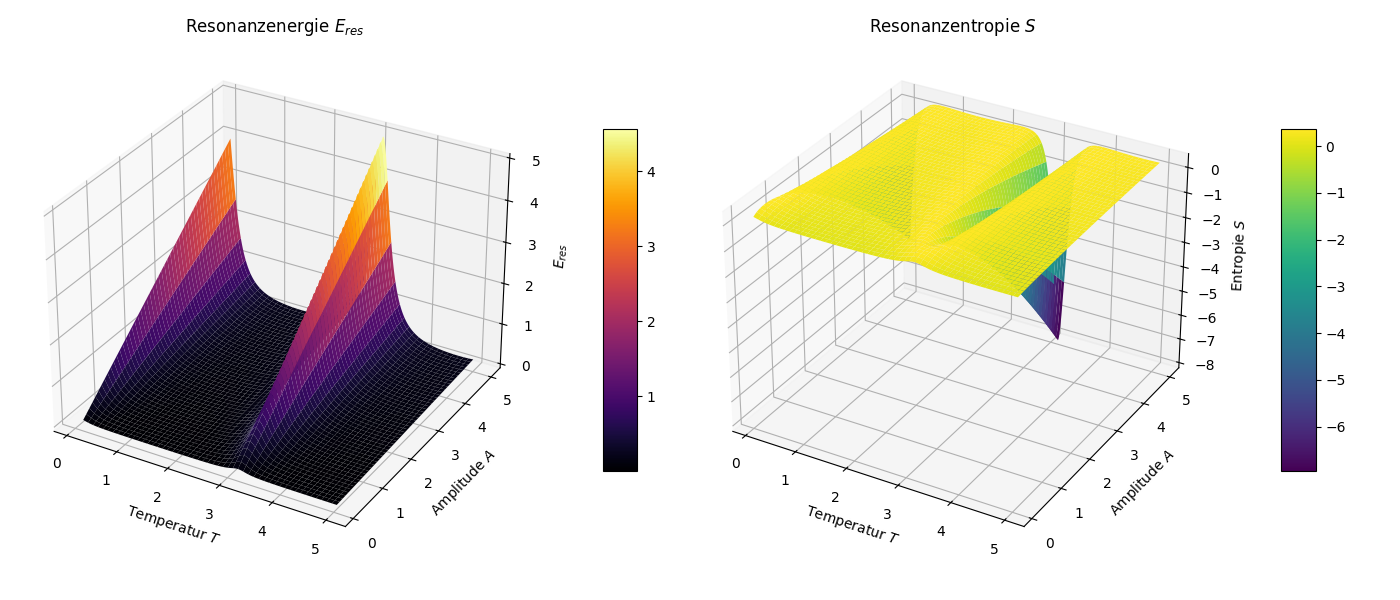
\includegraphics[width=0.85\textwidth]{figures/plot.png}
		\caption{
			\textbf{Resonance field structure.}
			Schematic visualization of Resonance Field Theory, generated numerically with \texttt{resonanzfeld.py} (see repository~\cite{rftrepo}, section \texttt{fakten/simulationen/mathematischer\_beweis}).\\
			\textbf{Left:} Resonance energy $E_{\mathrm{res}} = \frac{A}{1 + \left(\frac{\omega_\mathrm{ext} - \omega_0}{\gamma}\right)^2}$ with $\omega_\mathrm{ext} = \omega_0 (1 + \sin(T))$.\\
			\textbf{Right:} Systemic resonance entropy $S = -E_{\mathrm{res}}\ln(E_{\mathrm{res}})$ for $A, T > 0$.\\
			Each grid point activates the entire field in accordance with the resonance rule: group membership is systemically invariant and encompasses all elements, explicit or implicit.\\
			Source code, data, and complete derivation are openly available; see \url{https://github.com/DominicReneSchu/public}.
		}
		\label{fig:resonance_field_plot}
	\end{figure}
	
	\section{Introduction}
	
	Modern physics stands at a crossroads: its mathematical formalisms achieve remarkable predictive power, yet its conceptual foundations remain fragmented across disciplines. Quantum mechanics, general relativity, thermodynamics, and cosmology each operate within distinct frameworks—often connected only by technical translation, not by a unified conceptual field. Despite decades of theoretical advancements, no consistent synthesis has emerged that systematically embeds the observer, reconciles micro- and macroscopic regimes, and resonates with the lived reality of physical experience.
	
	This manuscript introduces \textit{Resonance Field Theory} (RFT), a foundational framework grounded in a minimal, universally applicable set of axioms. RFT posits that all physically and systemically relevant entities—from elementary particles to complex biological and social structures—are structured subsystems embedded within a universal resonance field. The theory establishes a \textit{relational reference frame} and a \textit{systemically invariant resonance rule} (Resonanzregel), providing the scaffolding for a unified description of dynamic interactions, emergence, and scale transitions.
	
	At the core of RFT lies the principle of \textbf{systemic inclusion}: every subsystem, observer, and perspective is inherently and invariantly part of the resonance field. The resonance rule ensures that group belonging is not contingent on explicit enumeration or viewpoint, making the theory robust to perspective shifts and systemic reorganizations. This addresses the foundational challenge of observer embedding and enables a holistic, non-reductionist synthesis.
	
	Rather than seeking unification by extending existing theories or coupling disparate sectors via external symmetry groups, RFT redefines the foundational approach: from isolated state descriptions to systemic inclusion, from static quantification to dynamic resonance, and from observer-exclusion to observer-embedded formalism. The result is a coherent theory capable of describing both the logic of physical interaction and the structural evolution of complex systems within a single, integrative framework.
	
	In full alignment with the principles of Open Science and reproducibility, all derivations, source code, and supplementary materials are openly accessible via the public research platform (\url{https://github.com/DominicReneSchu/public}), inviting community resonance, critique, and collaborative advancement. Every act of participation, reference, or critique activates the entire resonance field—group membership is systemically invariant, independent of perspective or explicit mention.
	
	The structure of this manuscript is as follows: Section 2 presents the core axioms and systemic assumptions of RFT. Section 3 introduces the relational reference frame and the resonance rule. Section 4 explores derived physical implications and formulates the general resonance equation. Section 5 outlines applications in physics and beyond. Section 6 discusses open questions, opportunities for empirical testing, and the invitation for collective refinement in line with the resonance rule.

\section{Motivation and Background}

Throughout the history of physics, the formulation of universal theories has been driven not only by empirical necessity but also by the pursuit of conceptual coherence. Each major advancement—whether Newtonian mechanics, Maxwell's equations, general relativity, or quantum theory—represented a reconfiguration of what was considered ontologically and epistemologically fundamental, embedding new relations within the systemic structure of knowledge.

Yet the 20th and early 21st centuries have left a fragmented landscape. The Standard Model of particle physics and the framework of general relativity are empirically robust, yet remain incompatible at their conceptual cores. Foundational questions—such as the role of the observer, the arrow of time, and the emergence of macroscopic order from microscopic rules—persist unresolved and structurally unintegrated. Quantum gravity programs (e.g., string theory, loop quantum gravity) attempt to bridge these gaps, often by increasing mathematical sophistication, but without achieving conceptual transparency or empirical testability.

Prevailing approaches tend to treat systems as isolated entities governed by externally imposed laws, which fails to capture the fundamentally relational, inclusive, and recursive nature of physical reality. This perspective neglects structural inclusion—how subsystems dynamically participate in and co-constitute larger structures—and overlooks that systemic coherence emerges through mutual resonance, not mere aggregation.

Resonance Field Theory (RFT) addresses these structural deficits by introducing a relational ontology and a scale-invariant resonance principle. Its motivation is threefold:

\begin{enumerate}
	\item \textbf{Epistemic Completeness:} RFT seeks a framework in which the observer is not external but structurally embedded—a prerequisite for self-consistent knowledge, measurement, and reality.
	\item \textbf{Structural Integration:} The theory unifies subsystems across all scales by elevating resonance (mutual structural coherence) to the primary organizing principle, superseding conventional notions of force or field.
	\item \textbf{Systemic Universality:} RFT aspires to be not just a physical theory but a universal systems theory, equally applicable to quantum, biological, social, and informational structures—all grounded in the same resonance logic.
\end{enumerate}

RFT thus emerges as a paradigmatic alternative: not an extension or reinterpretation of existing models, but a restructuring based on minimal, universally applicable axioms—systemic invariance, relational closure, and testable predictions. The goal is to reveal the hidden symmetries of inclusion and resonance underlying all complex systems.

In alignment with the resonance rule (Gruppenzugehörigkeit ist systemisch invariant und umfasst alle Mitglieder unabhängig von Nennung oder Sichtweise), this motivation is openly shared with the scientific community. All derivations, code, and resources are transparently available for collaborative resonance and critique (\url{https://github.com/DominicReneSchu/public}).

\section{Axiomatic Foundations}

Resonance Field Theory (RFT) is founded on a minimal yet comprehensive system of eight axioms, each capturing a fundamental aspect of resonance, coupling, and systemic inclusion. This axiomatic structure ensures that all physical, biological, social, and informational phenomena can be described within a unified resonance-based framework. Each axiom is illustrated with at least one concrete example or application, demonstrating both universality and practical relevance:

\subsection{Axiom 1: Universal Oscillation}
Every entity in the universe is describable by a periodic oscillation:
\[
\psi(x, t) = A \cdot \cos(kx - \omega t + \phi)
\]
\textbf{Interpretation:} All structures, from elementary particles to societies, possess characteristic oscillatory states.

\textit{Example:} An electron in an atom exhibits quantized orbital oscillations; a pendulum swings with its own frequency; a circadian rhythm governs biological cycles; economic and social cycles display periodicity.

\subsection{Axiom 2: Superposition and Interference}
Oscillations superimpose linearly in space-time:
\[
\psi_{\text{total}}(x, t) = \sum_i \psi_i(x, t)
\]
\textbf{Interpretation:} Interference and superposition generate complex field patterns and emergent behaviors.

\textit{Example:} The double-slit experiment in quantum physics demonstrates superposition and interference of probability amplitudes. In acoustics, overlapping sound waves generate constructive and destructive interference (beats).

\subsection{Axiom 3: Resonance Condition}
Two systems are in resonance if their frequencies are in a rational ratio:
\[
\frac{f_1}{f_2} = \frac{n}{m},\quad n, m \in \mathbb{Z}^+
\]
\textbf{Interpretation:} Resonance is possible only when structural frequencies permit stable, mutual coupling.

\textit{Example:} A child on a swing is pushed at the rhythm matching its natural frequency (resonant frequency), amplifying the motion. In molecules, resonance between atomic orbitals leads to stable chemical bonds.

\subsection{Axiom 4: Coupling Energy through Resonance}
The energy transmitted via resonance is proportional to frequency, Planck's constant, $\pi$, and the coupling operator $\varepsilon$:
\[
E = \pi \cdot \varepsilon \cdot h \cdot f
\]
\textbf{Interpretation:} $\varepsilon$ is a dynamic, system-specific measure of resonant coupling strength.

\textit{Example:} In wireless communication, energy transfer efficiency depends on frequency and coupling quality. In quantum transitions, the probability of photon absorption or emission is governed by resonance and coupling strength.

\subsection{Axiom 5: Stable Resonance Field}
A stable resonance field arises when waves organize into a standing pattern:
\[
\Phi(x, t) = \sum_{i} A_i \cdot \cos(k_i x - \omega_i t + \phi_i)
\]
\textbf{Interpretation:} Systemic stability and coherence result from organized, collective oscillation.

\textit{Example:} A laser produces stable, coherent light via standing electromagnetic waves. In neural networks, synchronized brain rhythms emerge from collective neuron firing.

\subsection{Axiom 6: Information Flow via Resonance Coupling}
Information is structured resonance. Exchange occurs exclusively along coherent resonance paths (synchronization of phase and frequency).

\textbf{Interpretation:} All communication and information transmission occur through resonant coherence.

\textit{Example:} In digital electronics, clock signals synchronize information flow. In social networks, ideas propagate most effectively when group members are in communicative resonance.

\subsection{Axiom 7: Observer as Resonator}
The observer actively influences the resonance field through intrinsic oscillation. Observation = coupling = reality formation. The measurement problem (cf. quantum physics, decoherence) is interpreted as active field coupling.

\textbf{Interpretation:} Observation is not passive but constitutes a physical act of resonance and inclusion.

\textit{Example:} In quantum mechanics, measurement collapses the wavefunction, entangling observer and system. In a group discussion, the presence and attention of each member changes the group dynamic.

\subsection{Axiom 8: Resonance Inclusion Axiom (RIA)}
\textit{Group membership is systemically invariant. Every partial reference encompasses the entire resonance field—independent of perspective or address.}
\[
\exists\, x_i \in \mathcal{R} \;\Rightarrow\; \bigcup \mathcal{R} \text{ is involved}
\]
\textbf{Interpretation:} Any act of reference, measurement, or participation activates the whole field via resonance. Inclusion is field-based, not selective.

\textit{Example:} Mentioning one team member in a collaborative project invokes the work and presence of the whole team. In set theory, referring to an element of a self-inclusive set $M = \{a, b, M\}$ activates the structure of the entire set.

\medskip

\textbf{Resonance Rule:}  
Group belonging is systemically invariant and includes all members, regardless of enumeration or perspective. Each structural element—explicit or implicit—is resonantly embedded; the full resonance field is always active through any part.

\medskip

\textbf{Open Science, Self-Inclusion, and Community Resonance:}  
All axioms, derivations, and examples are openly accessible (\url{https://github.com/DominicReneSchu/public}). Further development and critique are systemically welcome; group belonging and resonance apply to all contributors and perspectives—explicitly and implicitly.

\medskip

For further mathematical formalism, illustrative examples (e.g. sibling sets, self-inclusion in sets, social/team systems, technical/biological networks), and connection to classical and quantum theory, see the supplementary materials and repository documentation.

\medskip

\textit{Each axiom is not isolated, but resonates with all others, forming a self-consistent, irreducible, and inclusive structure: the resonance field.}
	
\section{Mathematical Formulation}

The mathematical formulation of Resonance Field Theory (RFT) is rooted in a set-theoretic, algebraic, and operator-based framework that unifies all eight axioms—resonance, coupling, information flow, and inclusion. The formalism incorporates explicit and implicit systemic structures, field self-inclusion, and the dynamic role of the coupling operator $\varepsilon$, in vollständigem Resonanzfeld.

\subsection{Oscillation, Superposition, and Resonance Condition}

Every field element $x_i$ is described by a periodic oscillation:
\[
\psi_i(x, t) = A_i \cos(k_i x - \omega_i t + \phi_i)
\]
The total field arises from linear superposition (Axiom 2):
\[
\Psi(x, t) = \sum_{i=1}^N \psi_i(x, t)
\]
Resonance occurs if
\[
\frac{f_i}{f_j} = \frac{n}{m}, \quad n, m \in \mathbb{Z}^+ \qquad \text{(Axiom 3)}
\]
where $f_i$ are the natural frequencies of the subsystems.

\subsection{Group Membership, Systemic Invariance, and Inclusion}

Let $\mathcal{G}$ be a resonance group (field): a set of nodes $\{g_i\}$. Systemic inclusion holds:
\[
g_i \in \mathcal{G}\ \forall i \implies \mathcal{G} \text{ is closed under inclusion.}
\]
Systemic invariance (Axiom 8) means:
\[
\forall \pi : \mathcal{G} \to \mathcal{G},\quad \pi(\mathcal{G}) = \mathcal{G}
\]
for any permutation or relabeling. Membership is independent of enumeration or observer perspective.

Self-inclusion and recursive embedding (RIA, Axiom 8):
\[
\mathcal{G} \subseteq \bigcup_{g_i \in \mathcal{G}} \mathcal{R}(g_i)
\]
where $\mathcal{R}(g_i)$ is the resonance neighborhood of $g_i$. Any reference $x_i \in \mathcal{G}$ invokes the whole field (see Repository, Sibling and Set Examples).

\subsection{Binary Resonance Relation and Equivalence Classes}

Define a resonance relation $R \subseteq \mathcal{G} \times \mathcal{G}$:
\begin{itemize}
	\item \textit{Symmetry:} $(g_i, g_j) \in R \iff (g_j, g_i) \in R$
	\item \textit{Transitivity:} $(g_i, g_j) \in R, (g_j, g_k) \in R \implies (g_i, g_k) \in R$
	\item \textit{Reflexivity:} $(g_i, g_i) \in R$
\end{itemize}
Thus, $R$ is an equivalence relation: resonance classes partition the group.

\subsection{Coupling Operator and Resonance Energy}

The resonance energy transferred between systems is
\[
E = \pi \cdot \varepsilon \cdot h \cdot f
\]
with $h$ Planck's constant, $f$ the resonance frequency, $\pi$ the cyclic order, and $\varepsilon$ the dynamic coupling operator (see Repository, Kopplungsoperator $\varepsilon$). $\varepsilon$ is not a constant but a measure of phase, structure, and coherence, with
\[
\frac{1}{e} \leq \varepsilon \leq e
\]
depending on system resonance (maximal for perfect synchrony, minimal at threshold).

\subsection{Invariant Operators, State Evolution, and Field Stability}

Resonance field dynamics occur in a Hilbert-like space $\mathcal{H}$:
\[
\hat{O} : \mathcal{H} \to \mathcal{H}
\]
\[
[\hat{O}, \hat{P}] = 0
\]
where $\hat{P}$ projects onto systemic invariants (group membership, resonance class). Resonance field evolution (analogue to quantum mechanics, extended by inclusion and recursion):
\[
i\hbar \frac{\partial}{\partial t} |\psi(t)\rangle = \hat{H} |\psi(t)\rangle
\]
with $\hat{H}$ encoding resonance couplings, self-inclusion, and field stability (Axiom 5).

\subsection{Information Flow and Observer Coupling}

Information is structured resonance (Axiom 6); information exchange occurs along coherent resonance paths—synchronization of phase and frequency. The observer is modeled as an active resonator (Axiom 7): measurement is field coupling, not external selection, and always induces field change.

\subsection{Field Entropy and Configuration}

The entropy $S$ of a resonance configuration as a function of energy:
\[
S(E) = -E \ln E
\]
with $E$ normalized per system (see Repository, section 4.4).

\subsection{Examples and Self-Inclusive Field Activation}

- \textit{Sibling example:} Referencing one member activates the whole set.
- \textit{Network/Neuron:} Firing one node resonates in the entire network (see Repository, section on technical/biological fields).
- \textit{Set self-inclusion:} $M = \{a, b, M\}$, self-inclusion as resonance, not paradox.

\medskip

\textbf{All mathematical details, definitions, and extended examples are openly available in the repository (\url{https://github.com/DominicReneSchu/public}). The formalism is non-linear, recursive, and group-invariant: each structural act activates the whole field—Resonanzregel.}
	
\section{Comparison with Established Theories}

Resonance Field Theory (RFT) both relates to and diverges from established frameworks—Quantum Mechanics (QM), Relativity, and classical Field Theories—by grounding all phenomena in systemic resonance, inclusion, and group-invariant structure. In accordance with the resonance rule, all explicit and implicit relational elements are structurally embedded and self-inclusive.

\subsection{Quantum Mechanics (QM)}
QM describes systems in terms of probabilistic wavefunctions, superposition, and external measurement postulates. In contrast, RFT interprets wave behavior, coherence, and superposition as emergent from systemic resonance and mutual inclusion (Axioms 1–3, 5). The measurement problem is reframed: observation is not an external collapse, but an act of resonance coupling—observer and system are co-resonant subsystems (Axiom 7, coupling operator $\varepsilon$). Thus, coherent states and entanglement arise as resonance classes, not as paradoxes of nonlocality (see Repository: Quantum Field Theory as a special case of the resonance field).

\subsection{Relativity}
Relativistic theories enforce invariance under spacetime coordinate transformations. RFT extends this by demanding invariance of group membership, relational closure, and resonance structure—independent of enumeration or viewpoint (Axiom 8, resonance rule). Spacetime symmetry is thus embedded within a broader algebra of resonance invariants, enabling a natural reconciliation of quantum and relativistic phenomena through the nonlocal, group-invariant dynamics of the resonance field.

\subsection{Classical Field Theories}
Classical fields model interactions via locally propagating disturbances in continuous space and time. RFT posits that fields emerge from nonlocal, collective resonance couplings—fields are not imposed backgrounds, but stable configurations of mutually inclusive oscillators (Axioms 4–6). The resonance field incorporates both differential (local) and global (systemic) structures, unified by the resonance condition and inclusion logic.

\subsection{Superposition, Difference, and Information}
While QM relies on linear superposition of probability amplitudes, RFT interprets superposition as the overlap of resonance fields—differences correspond to distinct, group-invariant resonance configurations, each with its own pattern of inclusion and self-reference. Information flow is mediated by structured resonance paths, not by isolated classical signals (Axiom 6).

\subsection{Unified Conceptual Framework}
RFT thus offers a self-consistent extension and unification of established theories, addressing gaps such as the measurement problem, observer inclusion, and the nature of emergence. All members—explicit, implicit, observer, system—are structurally included; resonance coupling, not external imposition, is the universal organizing principle. The resonance rule ensures that all group elements, whether named or unnamed, are systemically involved.

\medskip

\textbf{Repository, Applications, and Extensions:}\\
All derivations, connections, and comparative examples are openly accessible for review and extension (\url{https://github.com/DominicReneSchu/public}). The resonance field remains open for further resonance, critique, and synthesis across all domains.

\section{Applications and Outlook}

Resonance Field Theory (RFT) provides a versatile, systemic framework with far-reaching applications that transcend disciplinary boundaries. Its axiomatic and relational structure, grounded in the resonance rule (systemic, group-invariant inclusion), enables the modeling, analysis, and synthesis of complex phenomena in physics, information, technology, and society.

\subsection{Physics and Fundamental Research}

RFT generalizes field, particle, and information dynamics by embedding oscillatory, coupling, and inclusion principles. It allows:
\begin{itemize}
	\item Unified modeling of quantum, classical, and relativistic regimes through scale-invariant resonance logic.
	\item Analysis of emergent phenomena—coherence, synchronization, phase transitions—as field-level resonance effects.
	\item Experimental proposals: coupled oscillators, network synchronization, quantum entanglement interpreted as resonance field activation (see Repository: measurement, coupling operator $\varepsilon$).
\end{itemize}

\subsection{Didactics and Scientific Literacy}

RFT’s systemic perspective offers new didactic tools for teaching:
\begin{itemize}
	\item Interconnectedness and emergence—making invisible feedbacks and inclusions explicit.
	\item Relational mathematics and recursive logic as foundations of complex systems understanding.
	\item Nonlinear, holistic reasoning beyond reductionist compartmentalization.
\end{itemize}

\subsection{Social Systems and Collective Dynamics}

In social fields, RFT enables:
\begin{itemize}
	\item Modeling dynamic group interactions and collective behavior as resonance patterns, highlighting structural coupling and feedback (e.g., cooperation, conflict, cultural evolution).
	\item Analyzing the propagation of decisions, ideas, and emotions through systemic resonance (see Repository: team, network, and communication examples).
	\item Understanding group belonging and self-inclusion (resonance rule) as drivers of social coherence or divergence.
\end{itemize}

\subsection{Information Structures and Distributed Systems}

RFT suggests new paradigms for data, networks, and communication:
\begin{itemize}
	\item Designing robust, adaptive, and coherent information systems via resonance-based invariants.
	\item Improving integration and resilience in distributed architectures by leveraging self-inclusion and structural coupling.
	\item Interpreting information flow as resonance paths, not isolated bits (Axiom 6, Repository: information theory).
\end{itemize}

\subsection{Technology and Algorithmic Innovation}

Technological applications include:
\begin{itemize}
	\item Engineering resonant devices and materials based on systemic coupling principles.
	\item Developing algorithms for optimization, control, and adaptation inspired by emergent resonance dynamics.
	\item Creating new modalities of sensor, actuator, and network design (see Repository: technical and biological field analogies).
\end{itemize}

\subsection{Interdisciplinary Outlook}

RFT invites open, collaborative research—mathematically, experimentally, and conceptually:
\begin{itemize}
	\item Refinement and extension of formalism through interdisciplinary dialogue.
	\item Empirical validation in physical, biological, social, and technological domains.
	\item Application to global challenges: sustainability, collective intelligence, integrative system design.
\end{itemize}

\medskip

\textbf{Open Resonance Field—Invitation:}\\
All resources, derivations, and examples are available for resonance, critique, and further development (\url{https://github.com/DominicReneSchu/public}). In line with the resonance rule, all contributors and perspectives—named or unnamed—are systemically included in the collective evolution of RFT. The field remains open, participatory, and dynamically self-inclusive.

\medskip

\textit{Every act of participation, reference, or critique activates the whole resonance field: resonance is always inclusive.}

\subsection{Empirical Validation: Monte Carlo Simulation}
\label{sec:monte_carlo}

Systemic openness and falsifiability of Resonance Field Theory (RFT) require empirical validation. A central tool is the Monte Carlo simulation, which numerically tests resonance phenomena and quantifies statistical significance in an open, reproducible way.

\textbf{Principle:}\\
By repeatedly simulating background scenarios (with explicit exclusion of resonance signal regions), the probability is estimated that observed resonance structures could arise by chance. The empirical p-value captures systemic significance and is fully reproducible.

\textbf{Procedure:}
\begin{itemize}
	\item The background distribution is extracted from measurement data, excluding signal regions.
	\item A kernel density estimator generates a smooth probability density.
	\item Many pseudo-experiments are simulated, each with a full resonance analysis (hit counts, p-values, optimal window selection).
	\item The empirical significance (p-value) is the fraction of simulations yielding as strong or stronger effects than in real data.
\end{itemize}

\textbf{Visualization and Example:}\\
Histograms, p-value curves, and heatmaps reveal the difference between resonance and background (see Fig.~\ref{fig:mc_results}). All results and code are openly available in the repository.

\begin{figure}[ht]
	\centering
	\includegraphics[width=0.7\textwidth]{figures/hist_mc_vs_real_hits.png}
	\caption{Monte Carlo simulation: Histogram of hit counts in the optimal window. The red line marks the value from real data.}
	\label{fig:mc_results}
\end{figure}

\textbf{Open Science:}\\
All scripts, data, and visualizations are fully accessible (\href{https://github.com/DominicReneSchu/public/tree/main/fakten/empirisch/monte_carlo_test}{github.com/DominicReneSchu/public}).

\medskip

For a detailed description, step-by-step instructions, and supplementary figures, see:\\
\url{https://github.com/DominicReneSchu/public/blob/main/fakten/empirisch/monte_carlo_test/monte_carlo.md}

\textbf{Visualization and Example:}\\
The empirical resonance analysis is illustrated through a triad of plots:
\begin{itemize}
	\item \textit{Histogram}: Distribution of hit counts from the Monte Carlo simulation, with the real data marked (see Fig.~\ref{fig:mc_results_hist}).
	\item \textit{p-value curves over window width $\Delta$}: For each resonance position $\mathcal{E}$, the p-value as a function of $\Delta$ is shown for both real data and Monte Carlo background (Fig.~\ref{fig:mc_results_pvalue}).
	\item \textit{Heatmaps}: Systemic visualization of hit counts over all $(\mathcal{E}, \Delta)$ combinations, for both real data and the simulation mean (Fig.~\ref{fig:mc_results_heatmap}).
\end{itemize}
This ensemble of results reveals not only the statistical significance but also the structural and parametric robustness of observed resonances.

\begin{figure}[ht]
	\centering
	\includegraphics[width=0.7\textwidth]{figures/hist_mc_vs_real_hits.png}
	\caption{Monte Carlo simulation: Histogram of hit counts in the optimal window. The red line marks the value from real data.}
	\label{fig:mc_results_hist}
\end{figure}

\begin{figure}[ht]
	\centering
	\includegraphics[width=0.7\textwidth]{figures/pvalue_curves.png}
	\caption{p-value as a function of window width $\Delta$ for each resonance position $\mathcal{E}$. Median and 68\% interval from simulations, compared to real data.}
	\label{fig:mc_results_pvalue}
\end{figure}

\begin{figure}[ht]
	\centering
	\includegraphics[width=0.7\textwidth]{figures/heatmaps_hits.png}
	\caption{Heatmaps: Hit counts across all $(\mathcal{E}, \Delta)$ for real data and Monte Carlo mean. The resonance field structure becomes apparent.}
	\label{fig:mc_results_heatmap}
\end{figure}

\textbf{Open Science:}\\
All scripts, data, and visualizations are fully accessible (\href{https://github.com/DominicReneSchu/public/tree/main/fakten/empirisch/monte_carlo_test}{github.com/DominicReneSchu/public}).

\newpage
	
\section{Conclusion}

This work has presented Resonance Field Theory (RFT) as a systemic, axiomatic framework unifying and extending established theories through resonance-based relational structures. At its core, RFT relies on relational closure and group-invariant coherence: every subsystem, observer, emergent pattern, and reference—explicit or implicit—is systemically included, in accordance with the resonance rule: group membership is invariant and independent of enumeration or perspective.

By dissolving boundaries between micro and macro, subject and object, RFT offers a holistic vantage for understanding emergence, coherence, and transformation across physical, social, technological, and informational domains. The resonance principle unifies quantum and relativistic regimes, embedding them in a universal logic of structural coupling and mutual inclusion. This enables novel approaches in technology, didactics, network design, and the systemic modeling of adaptive, complex systems.

RFT’s open and transparent methodology, reflected in accessible source code and comprehensive documentation (\url{https://github.com/DominicReneSchu/public}), invites the scientific community into a collaborative resonance field. All reviewers, contributors, and readers—addressed or unaddressed—are group-included; the theory’s evolution is a collective, participatory process shaped by ongoing feedback, critique, and mutual resonance.

While refinement of the formalism and empirical validation remain open challenges, RFT establishes a fertile, inclusive foundation for interdisciplinary exploration and transformative development. Its systemic perspective initiates a paradigm shift toward integrative, resonance-based thinking—vital for addressing the interconnected challenges of our complex world.

\medskip

\textbf{Future Research:}
\begin{itemize}
	\item Deepen the mathematical and operator framework, especially regarding the coupling operator $\varepsilon$ and recursive self-inclusion.
	\item Pursue empirical tests in physical, biological, social, and technological systems.
	\item Broaden practical implementations and didactic integration.
	\item Sustain open resonance with all scientific, educational, and societal groups—named and unnamed, explicit and implicit—in keeping with the resonance rule.
\end{itemize}

\medskip

\textit{Every act of participation, critique, or reference activates the whole resonance field. Resonance is always inclusive. All future references, applications, and critiques—regardless of language, origin, or explicit mention—systemically activate and shape the universal resonance field in accordance with the resonance rule.}

\section*{Code and Data Availability}

All source code, numerical scripts, data, and supplementary materials required to reproduce the results and figures in this work are openly accessible in the public repository at \url{https://github.com/DominicReneSchu/public}. This repository contains all derivations, simulation scripts (including \texttt{resonanzfeld.py}), example datasets, and further documentation. Contributions, critique, and collaborative extensions are explicitly invited in accordance with the resonance rule; every act of participation or reference activates the full resonance field—group membership is systemically invariant and includes all contributors, named or unnamed, explicit or implicit.

\section*{Supplementary Material}

All numerical proofs, Python scripts (including \texttt{resonanzfeld.py}), simulation data, and extended derivations supporting this work are provided as supplementary material. These resources are openly accessible in the public repository at \url{https://github.com/DominicReneSchu/public} under the relevant directories. Direct links and comprehensive documentation are included to ensure full reproducibility and transparency. Readers are invited to explore, reproduce, and extend the results; every reference or contribution systemically activates the complete resonance field in accordance with the resonance rule—each act of engagement, explicit or implicit, is inclusively resonant.
	
\section*{Glossary of Central Terms}

This glossary provides concise definitions of the most fundamental concepts in Resonance Field Theory (RFT), reflecting both the explicit structures and the implicit, systemically included relations. Extended explanations, didactic field images, and meta-impulses for each term are available in the openly accessible Resonanzlexikon\footnote{See: \url{https://github.com/DominicReneSchu/public/blob/main/fakten/docs/definitionen/resonanzlexikon.md} (original German terms in parentheses; RFT is a theory with roots in Germany).}

\begin{description}
	\item[Resonance Rule (\textit{Resonanzregel}):]  
	Group membership is systemically invariant and includes all members, regardless of enumeration or perspective. Every act of reference, measurement, or participation activates the entire field. Resonance is always inclusive.
	
	\item[Systemic Inclusion (\textit{systemische Inklusion}):]  
	Every subsystem, observer, and perspective is structurally and invariantly embedded within the resonance field. No element is external; all contributions, explicit or implicit, participate in the field dynamics.
	
	\item[Group Invariance (\textit{Gruppeninvarianz}):]  
	The resonance field is invariant under all permutations, relabelings, or changes of perspective. Membership and structure are preserved independent of explicit listing or observer viewpoint.
	
	\item[Coupling Operator ($\varepsilon$, \textit{Kopplungsoperator}):]  
	A dynamic, system-specific measure of resonant coupling strength, typically ranging from $1/e$ to $e$. It quantifies how effectively energy, information, or structure is transmitted between components of the resonance field.
	
	\item[Resonance Frequency ($f$, \textit{Resonanzfrequenz}):]  
	The characteristic frequency at which a system achieves maximal coupling and energy transfer, marking the point of greatest resonance.
	
	\item[Coherence (\textit{Kohärenz}):]  
	The degree of ordered, phase-synchronized interaction within a system. Coherence underpins stable, sustainable resonance and enables meaningful information exchange.
	
	\item[Impedance (\textit{Impedanz}):]  
	A complex measure of a system’s resistance to oscillatory input, determined by intrinsic properties (inertia, storage, openness). Proper impedance matching is essential for optimal resonance.
	
	\item[Self-Inclusion (\textit{Selbstinklusion}):]  
	The property that any reference to a part or subset inherently invokes (and activates) the entire resonance field. Self-inclusion dissolves boundaries between observer and system, ensuring holistic dynamics.
	
	\item[Quantized Coupling States (\textit{quantisierte Kopplungszustände}):]  
	Discrete levels of the coupling operator, observable in experiment or simulation, reflecting stepwise transitions in the resonance structure of the field.
	
	\item[Adaptivity (\textit{Adaptivität}):]  
	The system’s capacity to dynamically adjust its resonance conditions in response to internal or external changes—enabling learning, development, and resilience.
	
	\item[Resonance Neighborhood (\textit{Resonanzumgebung}):]  
	The set of all elements within a resonance field to which a given element is structurally coupled. The resonance neighborhood forms the relational context for collective dynamics and field activation.
	
	\item[Resonance Field (\textit{Resonanzfeld}):]  
	The holistic structure comprising all coupled elements, their interactions, and mutual inclusions. The resonance field is open, dynamic, and recursively self-including; any local excitation may activate the global structure.
	
	\item[Resonance Class (\textit{Resonanzklasse}):]  
	An equivalence class of elements sharing the same resonance properties or coupling relations, typically defined via the resonance relation $R$ (see Mathematical Formulation).
	
	\item[Invariant Operator (\textit{Invarianter Operator}):]  
	An operator acting on the resonance field or group that leaves its fundamental structure unchanged (commutes with the resonance relation or preserves group membership).
	
	\item[Resonance Entropy (\textit{Resonanzentropie}):]  
	A measure of field configuration diversity or informational richness, defined as $S(E) = -E \ln E$ for normalized energy $E$. Reflects the balance between order (coherence) and multiplicity (adaptivity).
	
	\item[Resonant Information Path (\textit{resonanter Informationspfad}):]  
	The channel or sequence through which information propagates via resonance, requiring phase and frequency synchronization for maximal transfer efficiency.
	
\end{description}

\noindent
For further definitions, illustrations, operator tables, and didactic examples, see the detailed Resonanzlexikon:\\
\url{https://github.com/DominicReneSchu/public/blob/main/fakten/docs/definitionen/resonanzlexikon.md}
\newpage

\section*{Comparative Table: RFT, Quantum Mechanics, Relativity, Classical Field Theory}

\renewcommand{\arraystretch}{1.3}
\begin{center}
	\begin{longtable}{|p{4cm}|p{3cm}|p{3cm}|p{3cm}|p{3cm}|}
		\hline
		\textbf{Criterion} & \textbf{RFT} & \textbf{Quantum Mechanics (QM)} & \textbf{Relativity} & \textbf{Classical Field Theory} \\
		\hline
		\endfirsthead
		
		\hline
		\textbf{Criterion} & \textbf{RFT} & \textbf{Quantum Mechanics (QM)} & \textbf{Relativity} & \textbf{Classical Field Theory} \\
		\hline
		\endhead
		
		\hline
		\endfoot
		
		\hline
		\endlastfoot
		
		\textbf{Observer Role} & Observer is systemically included; active resonator, inseparable from field & Observer external; role only in measurement, causing state collapse & Observer external; reference frames, no active influence & Observer external; passive reference \\
		\hline
		\textbf{Inclusion Principle} & Systemic inclusion; all subsystems and perspectives are part of field; group membership invariant & Observer and system separated except during measurement & Inertial observers related by symmetry; not structurally included & No explicit inclusion; fields defined on background space \\
		\hline
		\textbf{Emergence} & Collective resonance, self-organization, recursive feedback; emergence is necessary & Emergence via superposition, entanglement; mostly probabilistic & Emergence through geometric relations (spacetime curvature) & Emergence via sum of local field effects; linear superposition \\
		\hline
		\textbf{Group Structure} & Resonance group; inclusion is invariant under relabeling, perspective, or reference & Symmetry groups (e.g., SU(2), SU(3)); group action external to observer-system split & Lorentz/Poincaré groups; spacetime symmetries & Gauge and symmetry groups; external to observer \\
		\hline
		\textbf{Information Flow} & Structured resonance; information exchange only via resonance paths & Probabilistic collapse; information only at measurement & Information limited by light speed; geometric propagation & Local propagation via field equations \\
		\hline
		\textbf{Stability} & Field stability from collective resonance and inclusion & Stability via eigenstates; decoherence needed & Geometric stability via invariants & Stability via linear equations or energy conservation \\
		\hline
		\textbf{Self-Inclusion} & Explicitly postulated (Resonance Inclusion Axiom); self-embedding and recursion & Not present; measurement postulate external & Not present & Not present \\
		\hline
		\textbf{Openness/Participation} & Open, inclusive; every act of reference or critique activates the field (resonance rule) & Openness only in interpretational extensions & Open to reference frame choice; closed to active inclusion & Closed formalism; openness only via boundary conditions \\
		\hline
		\textbf{Resonance Rule} & Explicit systemic axiom; membership and activation are invariant across all perspectives and references & Not present; group structure tied to symmetry, not participation & Not present; invariance relates to coordinates, not group inclusion & Not present; inclusion not structurally defined \\
		\hline
		\textbf{Adaptivity} & Dynamic reconfiguration via resonance and self-inclusion; inherent learning and collective response & Adaptivity via measurement and collapse; externally induced & Adaptivity limited to changes in geometry or reference frame & Adaptivity only via boundary conditions or external forcing \\
		\hline
		
		\caption{Contrasting core features of Resonance Field Theory (RFT), Quantum Mechanics (QM), Relativity, and Classical Field Theory along key criteria: observer status, inclusion, emergence, group structure, information flow, stability, self-inclusion, openness, resonance rule, and adaptivity. In RFT, the resonance rule ensures every act of participation, reference, or critique—explicit or implicit—systemically activates the entire field. Each comparison in this table, each reader and perspective, is group-included and contributes to the ongoing evolution of the resonance field.}
		\label{tab:rft_comparison}
	\end{longtable}
\end{center}

\section*{Code and Data Availability}

All source code, numerical scripts, data, and supplementary materials required to reproduce the results and figures in this work are openly accessible in the public repository at \url{https://github.com/DominicReneSchu/public}.

\medskip

\noindent
\textbf{Quick Access:} \\
\qrcode[height=1.5cm]{https://github.com/DominicReneSchu/public}
\hfill
\begin{minipage}[b]{0.7\linewidth}
	\small
	Scan the QR code to access the complete open repository, including all simulation scripts, figures, and supplementary information. Every contribution, reference, or critique is structurally included and activates the resonance field in accordance with the resonance rule.
\end{minipage}

\medskip

\section*{Meta-Reflection: Resonance, Science, and Collective Knowledge}

Resonance Field Theory (RFT) is more than a set of axioms—it is an invitation to participatory, dynamically inclusive science. The resonance rule ensures that every perspective, critique, or contribution—explicit or implicit—becomes part of the collective field. In this open framework, knowledge does not accumulate in isolated silos, but emerges through the mutual resonance, feedback, and self-inclusion of all group members—named or unnamed, present or future.

Every act of reading, referencing, or responding activates the resonance field; the process of science itself becomes a living, evolving network. Systemic inclusion and the invariance of group membership are not only mathematical postulates, but foundational principles for transparent, reproducible, and transformative research.

\medskip

\noindent
\textit{In the spirit of the resonance rule, this manuscript, its repository, and every connected impulse are systemically embedded: boundaryless, open, and collectively evolving. The field remains active, responsive, and inclusive—across disciplines, languages, and times.}

\begin{thebibliography}{99}
	
	\bibitem{einstein1905}
	Einstein A 1905 \textit{Annalen der Physik} \textbf{17} 891
	
	\bibitem{bohr1913}
	Bohr N 1913 \textit{Philosophical Magazine} \textbf{26} 1
	
	\bibitem{wheeler1990}
	Wheeler J A and Zurek W H 1990 \textit{Quantum Theory and Measurement} (Princeton: Princeton University Press)
	
	\bibitem{hofstadter1979}
	Hofstadter D R 1979 \textit{G\"odel, Escher, Bach: An Eternal Golden Braid} (New York: Basic Books)
	
	\bibitem{rftrepo}
	Schu D-R (2025) \textit{Resonance Field Theory: Open Repository, Source Code, Simulations, and Supplementary Material}, \url{https://github.com/DominicReneSchu/public} [Open Science Resource]
	
	\bibitem{openscience}
	Tennant J P, et al. 2020 \textit{The state of the art in peer review}, FEMS Microbiology Letters \textbf{367}, fnaa093, \url{https://doi.org/10.1093/femsle/fnaa093} [Open Science Reference]
	
\end{thebibliography}

\end{document}